\documentclass{article}
    \usepackage[margin=0.8in]{geometry}
    \usepackage[parfill]{parskip}
    \usepackage[utf8]{inputenc}
    \usepackage{graphicx}
    \usepackage{siunitx}


\begin{document}
Excercise 1 \\
Rendell Cale, \today 

\section*{Question 1}
\begin{centering}
    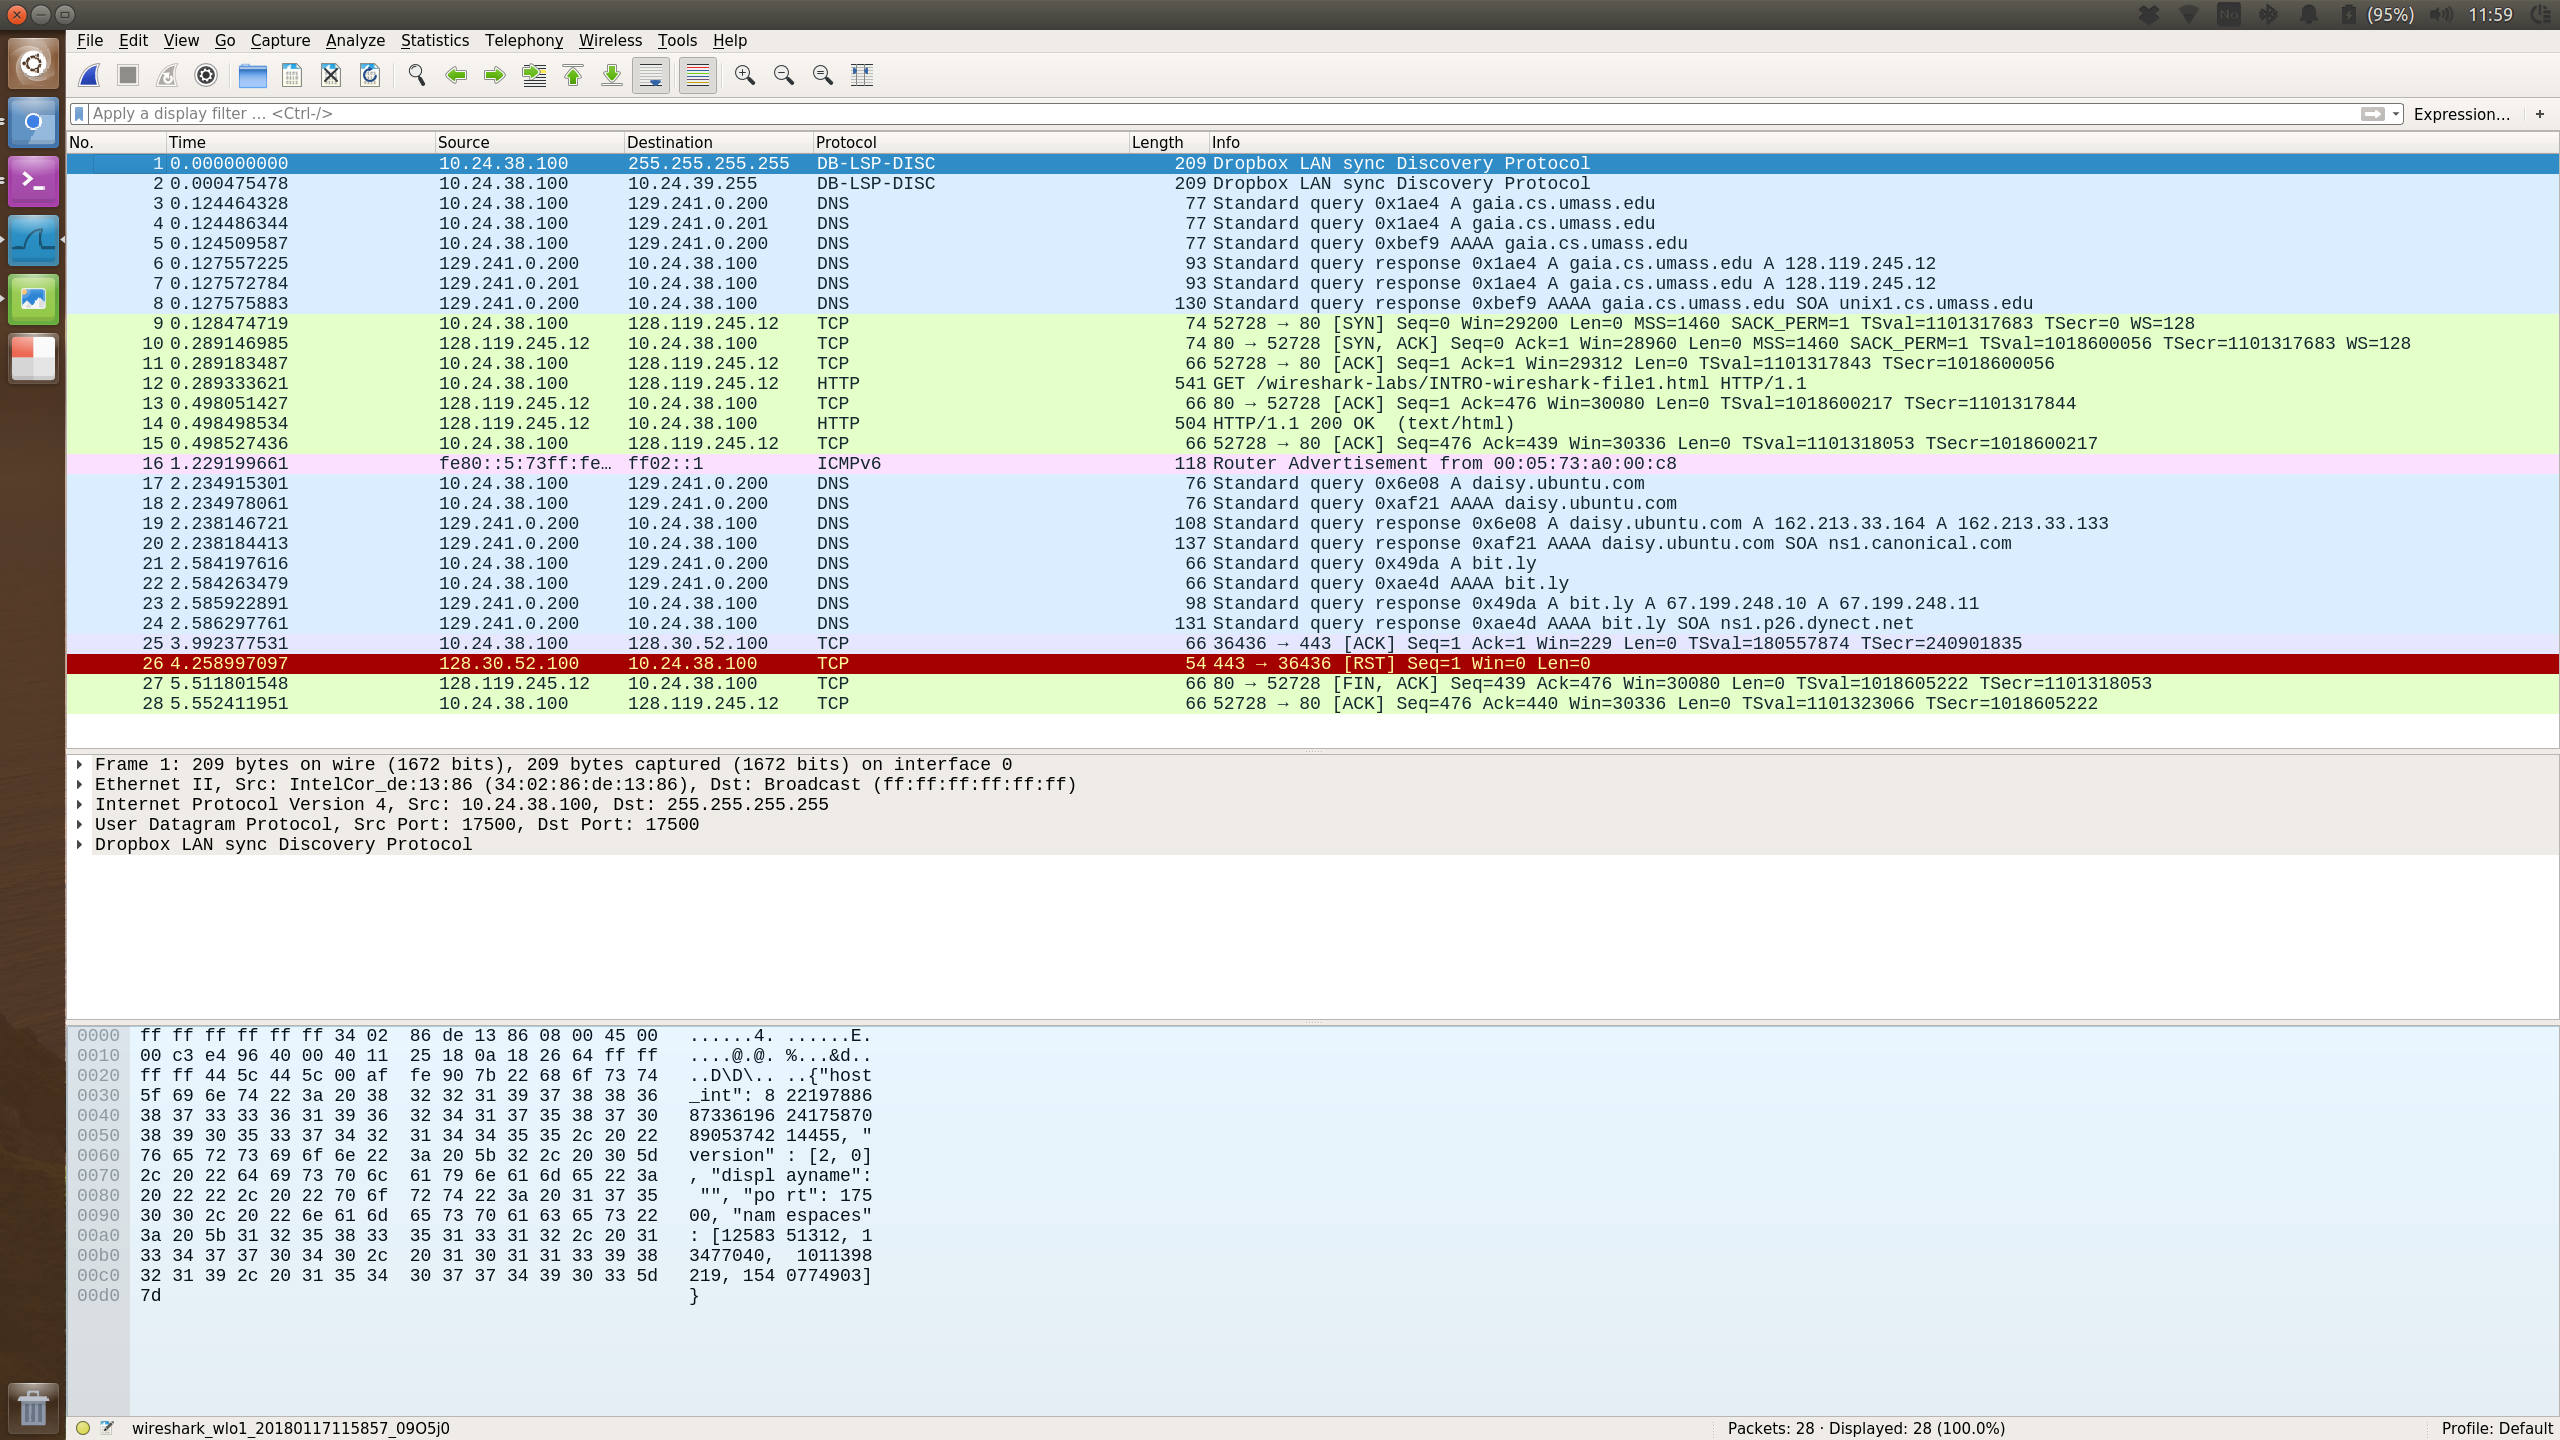
\includegraphics[width=\linewidth]{wireshark-intro.png}
\end{centering}
Looks like the three protocols related to the website access are:
\begin{itemize}
   \item DNS
   \item HTTP
   \item TCP
\end{itemize}


\section*{Question 2}
\begin{centering}
    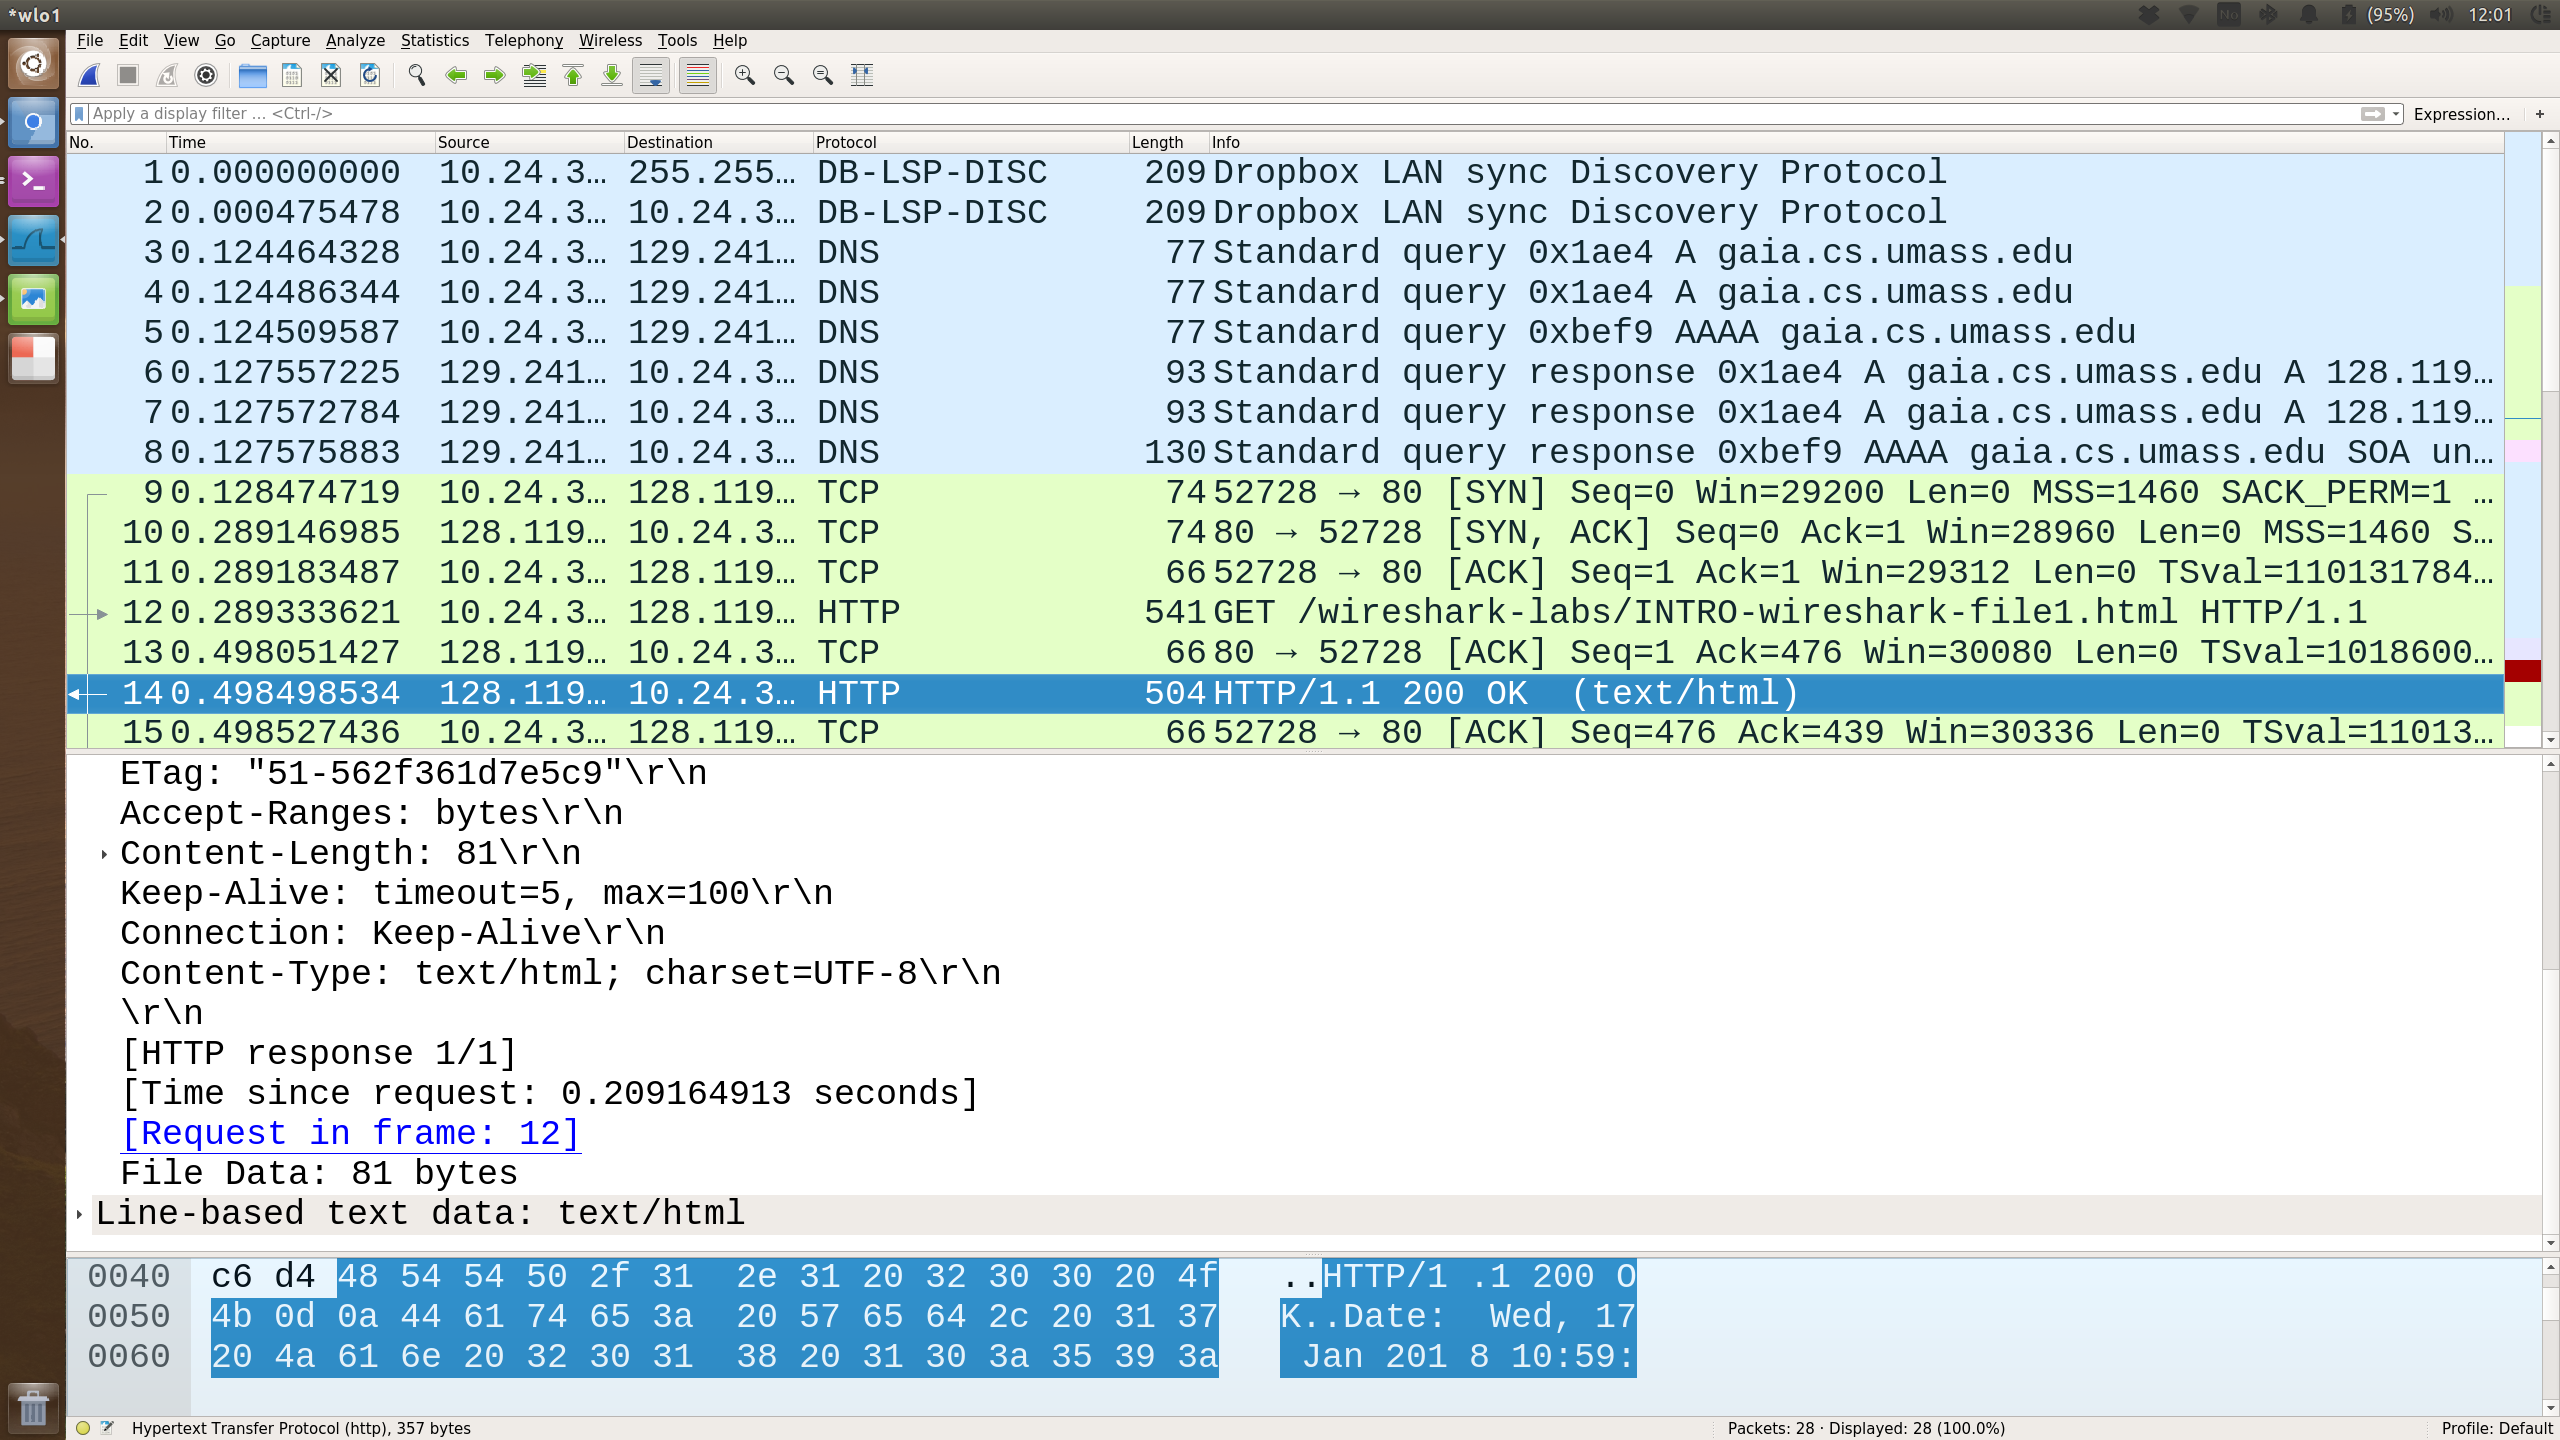
\includegraphics[width=\linewidth]{wireshark-intro-time.png}
\end{centering}
Going into to response entry, we can see that the time passed since request was about $\SI{0.2092}{\second}$. 

\section*{Question 3}
Looking at the source and destination of the HTTP GET request, we see that the source (my computer) has internet address 10.24.38.100 and that the website has internet address 128.119.245.12.


\section*{Question 4}
\begin{figure}[h]
    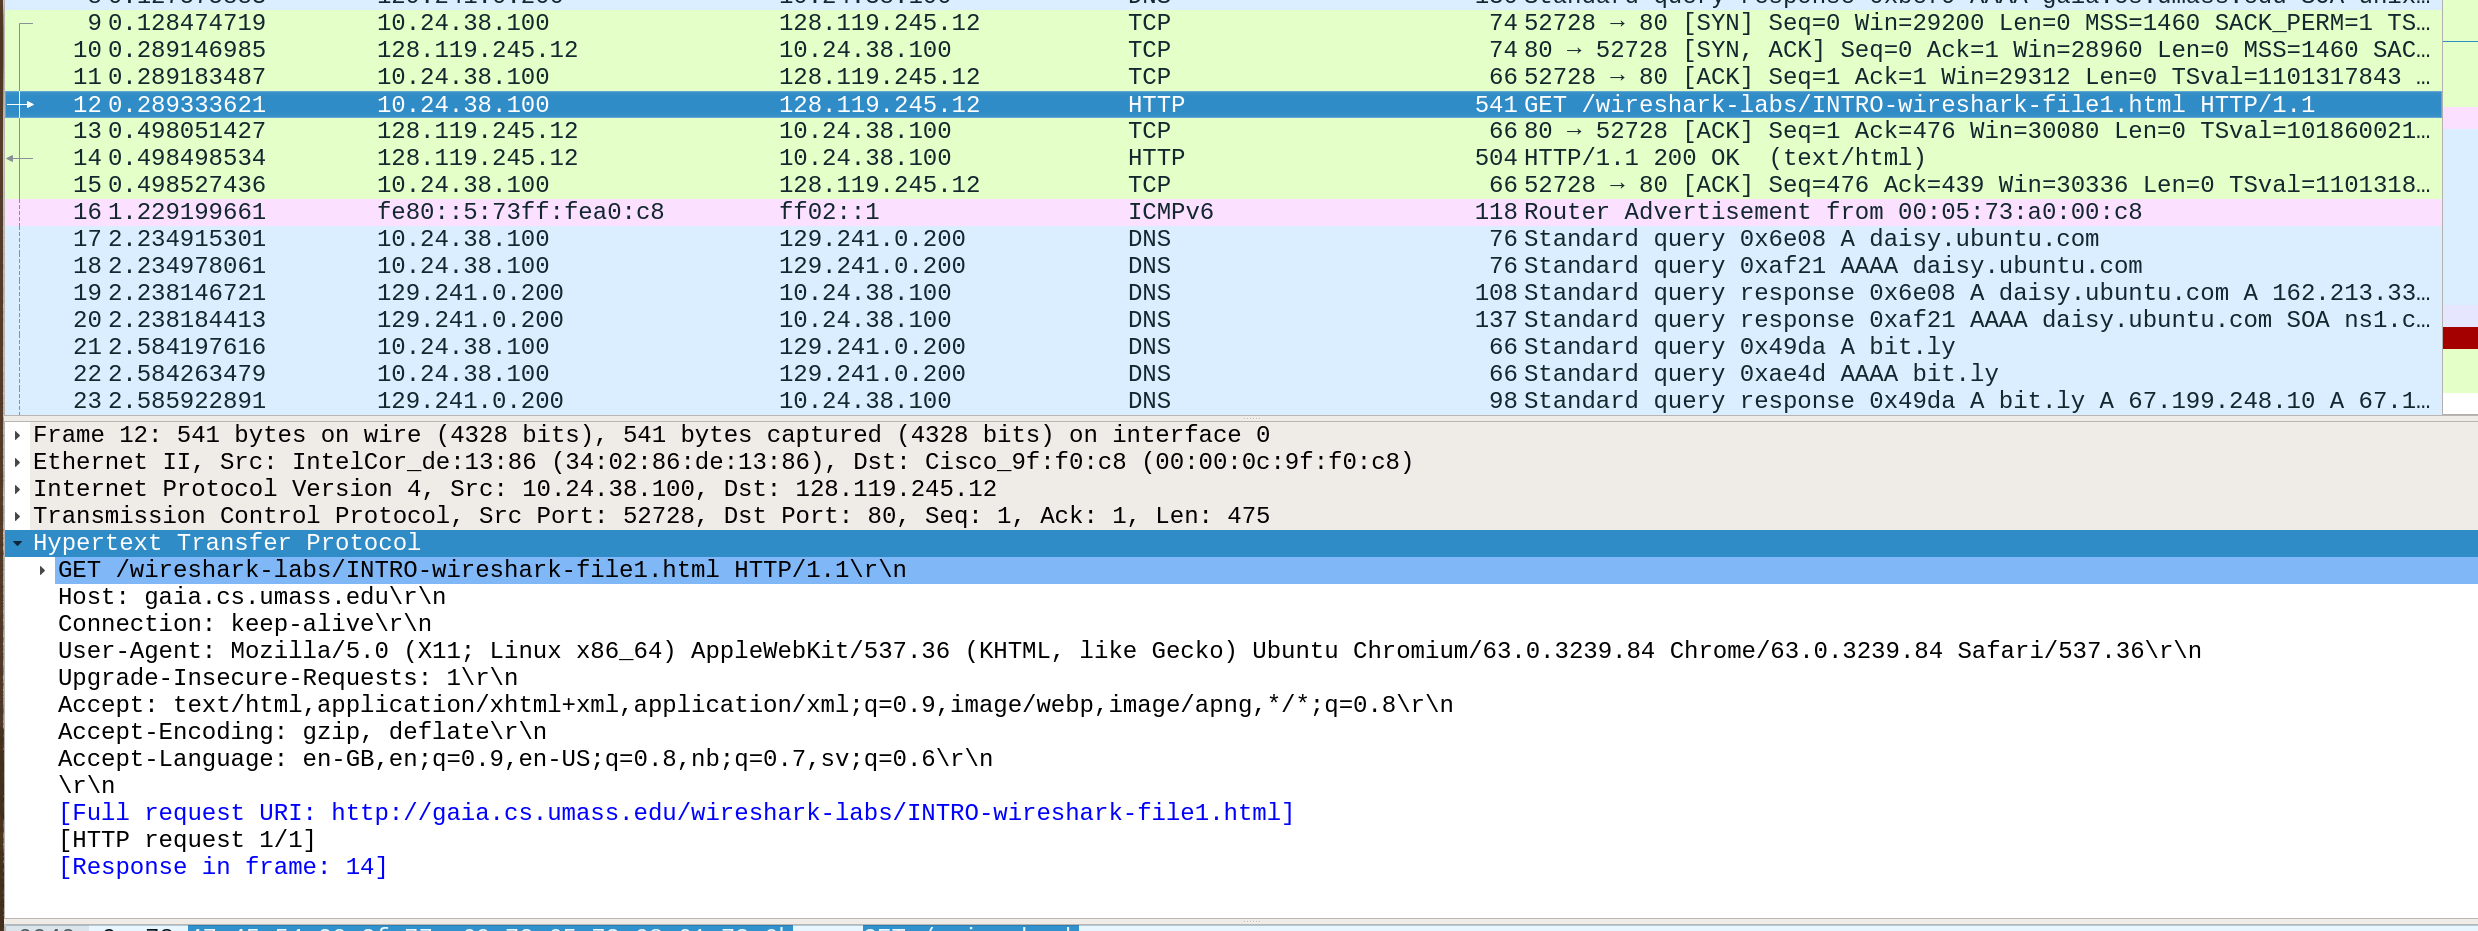
\includegraphics[width=\linewidth]{wireshark-intro-httpget.png}
    \caption{HTTP GET}
\end{figure}
\begin{figure}[h]
    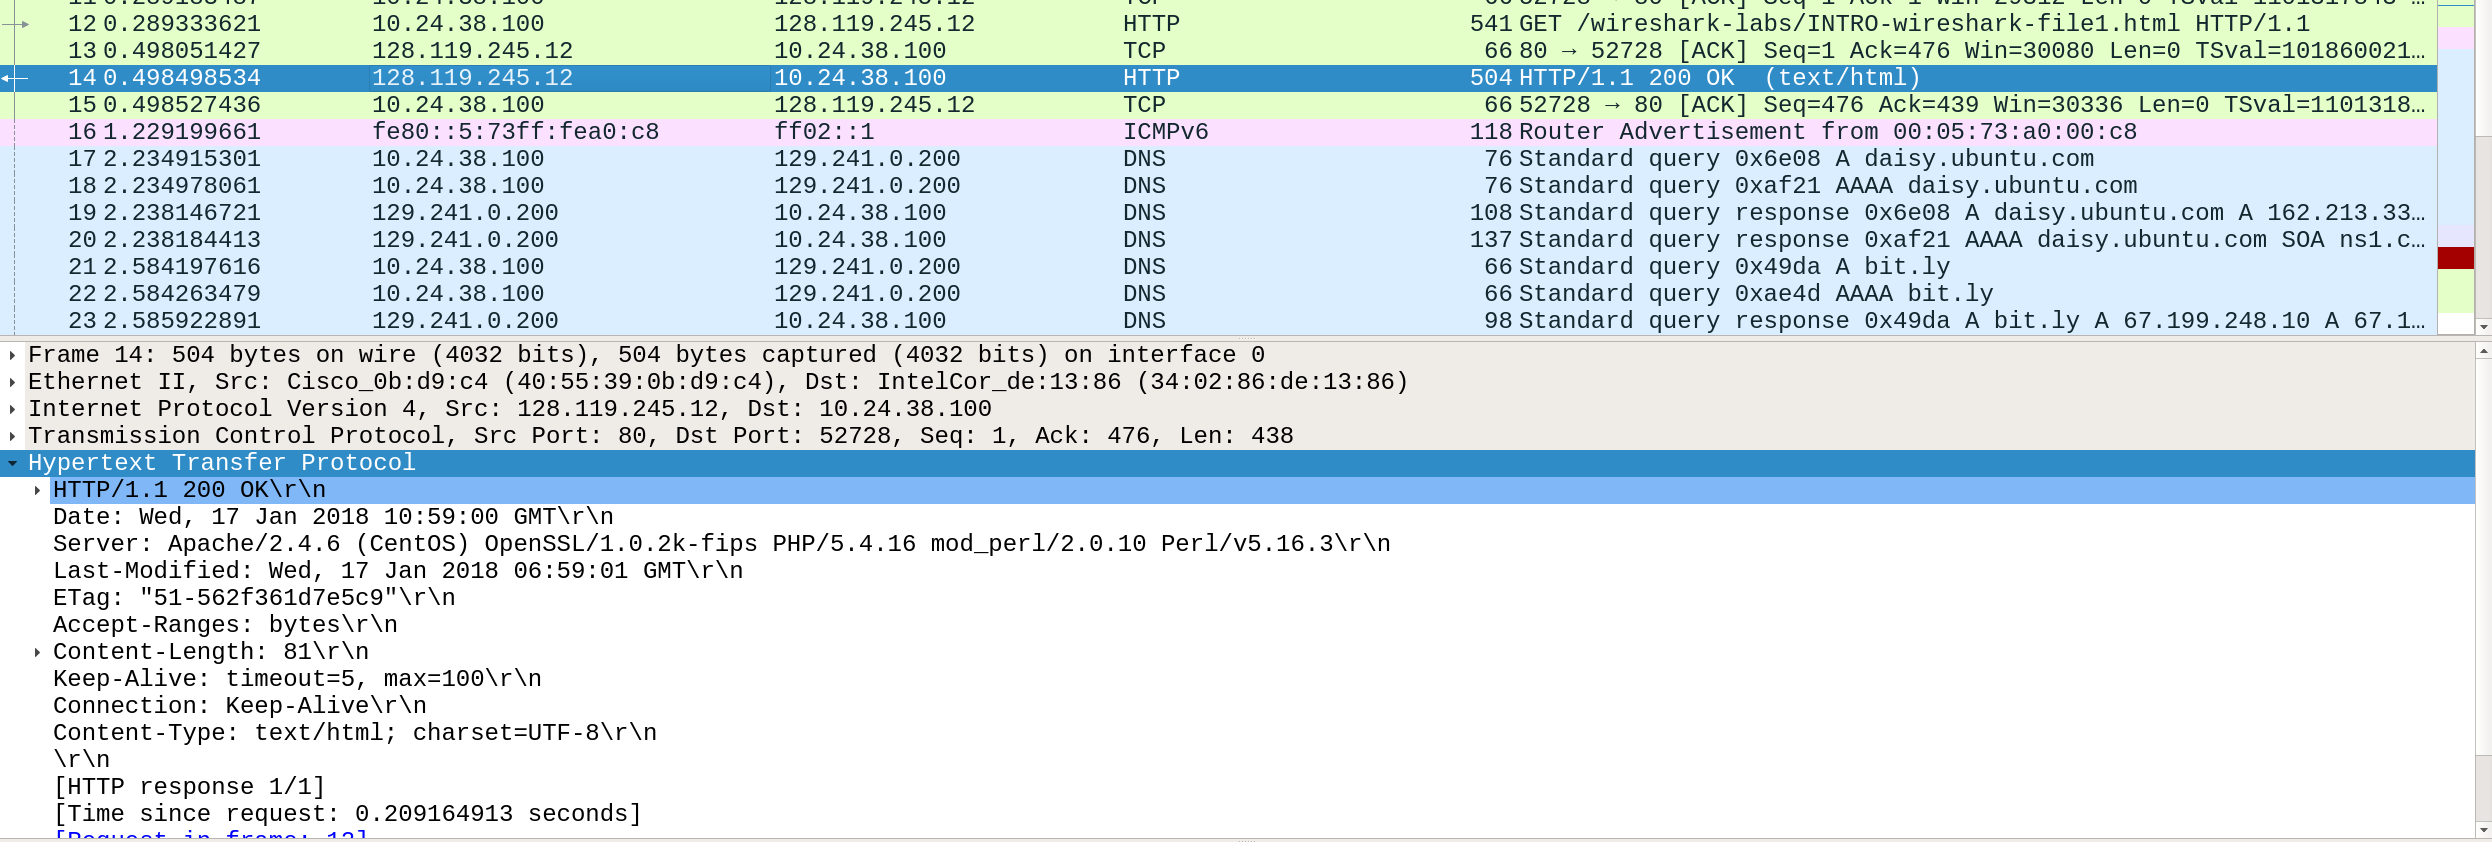
\includegraphics[width=\linewidth]{wireshark-intro-httpok.png}
    \caption{HTTP OK}
\end{figure}

\end{document}
